\documentclass[12pt, a4paper]{article}
    \usepackage[utf8x]{inputenc}
    \usepackage[russian]{babel}
    \usepackage{mathtools}
    \usepackage{graphicx}
    %\usepackage{minted}
    \usepackage{listings}
	\usepackage{xcolor}
    \usepackage[outputdir=out,cache=false]{minted}
    \addtolength{\topmargin}{-3cm}
    \addtolength{\textheight}{3cm}
    \lstset { %
    language=C++,
    backgroundcolor=\color{black!4}, % set backgroundcolor
    basicstyle=\footnotesize,% basic font setting
	}
\usepackage{amsmath}
\usepackage{graphicx}
\usepackage{braket}
\usepackage{amssymb}
\begin{document}`
\thispagestyle{empty}
\begin{center}
\ \vspace{-2cm}

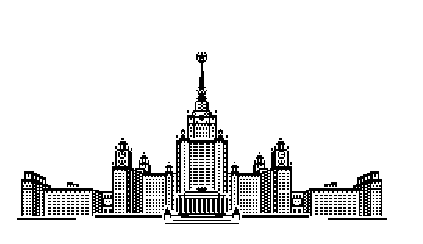
\includegraphics[width=0.5\textwidth]{msu.eps}\\
{\scshape Московский государственный университет \\ имени М.В.~Ломоносова}\\
Факультет вычислительной математики и кибернетики\\
Кафедра суперкомпьютеров и квантовой информатики

\vspace{3cm}

{\LARGE Выпускная квалификационная работа}

\vspace{1cm}

{\Huge\bfseries
<<Компьютерная химия малых ансамблей одновалентных искусственных атомов в модели Борна-Оппенгеймера>>\\}
\end{center}
\vspace{3cm}
\vfill

\begin{flushright}
  \large
  \textbf{Выполнил:}\\
  Студент 423 группы\\
  Грабовский~Максим~Михайлович

  \vspace{5mm}

  \textbf{Научный руководитель:}\\
  д.ф.-м.н., профессор\\
  Ожигов~Юрий~Игоревич
\end{flushright}

\vfill

\begin{center}
Москва, 2022
\end{center}
\enlargethispage{4\baselineskip}
\newpage

\tableofcontents
\newpage
\section{Введение}
\subsection{Введение}
\qquad Ансамбль одновалентных искусственных атомов в модели Борна-Оппенгеймера - это система, состоящая из нескольких искусственных атомов, каждый из которых имеет способен связаться с одним из атомов образовав молекулу.
\newline \null 
\qquad В такой системе можно изучать различные явления, связанные с квантовой механикой, такие как квантовые фазовые переходы, колебания и распространение волн в кристаллических структурах и т.д. 
Такие системы используются в квантовых вычислениях, где квантовые свойства ансамбля искусственных атомов могут быть использованы для решения определенных вычислительных задач.
\section{Поставновка задачи}
\subsection{Постановка задачи}
\qquad В данной работе проведено исследование неунитарной динамики квантовых состояний ансамблей одновалентных искуственных атомов в решетках в модели Борна-Оппенгеймера.
\section{Математические модели и методы}

\subsection{Уравнение Шредингера}
\qquad Уравнение Шредингера - главное уравнение квантовой механики, описывающее унитарную динамику квантовой системы, в данной работе будет моделироватся преимущественно неунитарная динамика, об этом далее.\newline
Уравнение Шредингера имеет вид:
\[i\hbar\ket{\dot\Psi}=H\ket{\Psi}\]
Где:\newline
$H$ - Оператор полной энергии системы, \newline
$\Psi$ - Вектор состояния,\newline
$\hbar$ - Приведённая постоянная Планка $= \frac{h}{2pi}$, где $h$ - постоянная Планка,\newline
$\dot\Psi$ - $\frac{\partial \Psi(x)}{\partial t}$. \newline \null\qquad
Выведем уравнение Шредингера для матрицы плотности:\newline
Для этого возьмём сопряжение уравнения и применим формулу дифференцирования произведения.
\[\bra{\Psi(t)}H=i\hbar\bra{\dot\Psi(t)}\]
\[\dot\rho=\bra{\dot\Psi}\ket{\Psi}+\bra{\Psi}\ket{\dot\Psi}\]
\[i\hbar\dot\rho(t)=[H,\rho]\]
Где:\newline $\rho$ - матрица плотности, \newline Коммутатор $[H,\rho]=H\rho-\rho H$.\newline
\\ 
\null\qquad Уравнение Шредингера позволяет моделировать ислючительно унитарную динамику, для изучения неунитарной (неэрмитовой, без требования к обратимости) динамики системы введём оператор декогеренции $\mathcal{L}(\rho)$ имеющий вид: \[\mathcal{L}(\rho)=\sum_{j=1}^N\gamma_j(A_j\rho A^*_j-\frac{1}{2}\{\rho,A_j^*A_j\})\]
Где:\newline
$\mathcal{L}$ - оператор Линдблада,\newline 
$A_j$ - факторы декогерентности,\newline 
$\rho$ - матрица плотности,\newline 
$A^*_j$- сопряженный $A_j$, \newline
Антикоммутатор $\{\rho,A^*A\}=\rho A^*A+A^* A\rho$.
\newline \null\qquad
Прибавив к уравнению Шредингера оператор декогеренции домноженный на $i$ получим уравнение вида:\[i\hbar\dot\rho(t)=[H,\rho]+i\mathcal{L}(\rho)\]
называемое уравнением Горини — Коссаковского — Сударшана (уравнением Линдблада) численное решение данного уравнение является основным методом моделированиея в данной работе.

\subsection{Уравнение Горини — Коссаковского — Сударшана (Линдблада)}
Уравнение Линдблада вида:
\[i\hbar\dot\rho(t)=[H,\rho]+i\mathcal{L}(\rho)\]
\qquad Является одним из основных инструментов в квантовых вычислениях. Оно описывает динамику квантовых систем при взаимодействии с окружающей средой, с наличием факторов декогеренции.
\newline
\null
\qquad
Уравнение Линдблада моделирует изменение квантовой системы со временем через вектор состояния, который задает вероятность нахождения системы в одном из возможных состояний . Взамиодействие с окружающей средой описывается через оператор Линдблада который моделирует действие окружающей среды на систему.
\section{Компьютерное моделирование}
\subsection{Задача}
\qquad В данной работе будем исследовать эволюцию системы $M$ искуственных атомов в трёхмерной решётке $N*N*N$, в модели атомы тунелируют внутри решетки, строго по прямоугольным рёбрам решетки, причём узел тунелирования должен быть не занят. При приближении двух атомов друг к другу с некой вероятностью может образоватся молекула. Расчёт квантовой ассоциации и диссоциации будем производить с допущением что в течении промежутка моделирования атомы неподвижны, рассматривать ассоциацию-диссоциацию будем как для системы двух неподвижных атомов. При ассоциации энергия связи будет выделятся в виде фонона возбуждения и уносится им, что и является фактором декогерениции. Фонон - квант механического колебания среды, в нашем случае решетки.
\newline
Закодируем состояния в виде вектора следующим образом:
\[\ket{at_0x\ \ at_0y\ \ at_0z}...\ket{at_{(M-1)x}\ at_{(M-1)y}\ at_{(M-1)z}} \ket{ph_x \ ph_y \ ph_z}\ket{cov_{0,1}..cov_{0,M-1}}\]
Где:\newline
$at_{n(x/y/z)}$ - координата n-го атома по оси, $at_{n(x/y/z)}\in[0,N-1]$,\newline
$at_{x/y/z}$ - фононы соответствующих осей, \newline 
$cov_{(x,y)}$ - ковалентная связь между атомами $x,y\in[0,M-1]$ 
\newline \null\qquad Число состояний такой системы будет превышать $M^4N^3$, что трудновычислимо, сократим число состояний системы зафиксировав позиции некоторых частиц и исключив недостижимые, пример (рис.1), 
\begin{figure}[htp]
\centering
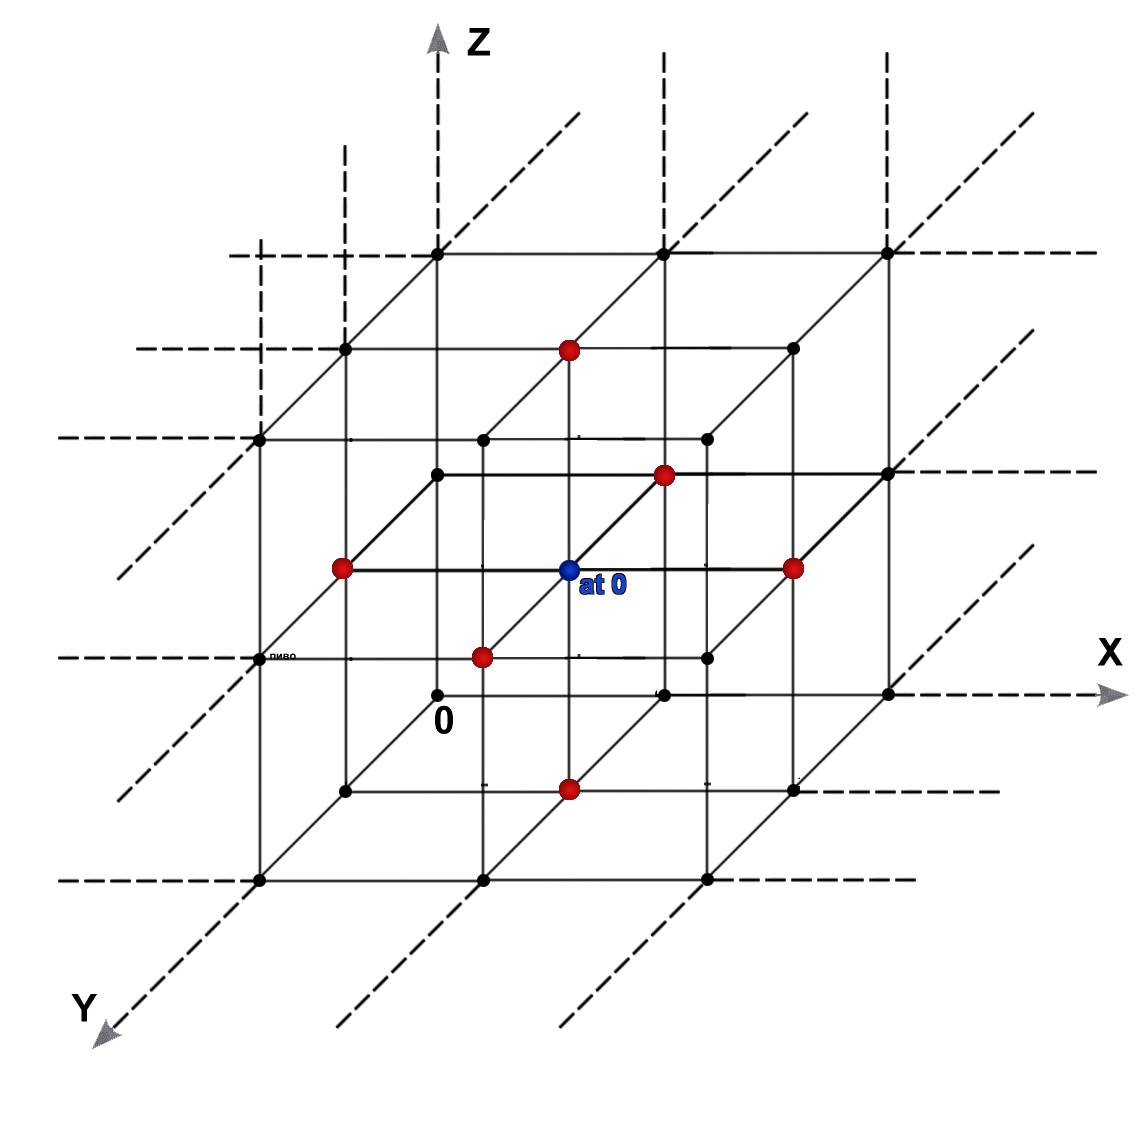
\includegraphics[scale=10.00]{area.png}
\caption{}
\label{}
\end{figure} 
\newline\null\qquad
Рассмотрим область размера 3*3 решётки, рассмотрим систему координат относительно этой области, зафиксируем позицию атома $at_0$ в точке $(1,1,1)$, тогда образование молекулы возможно только при появлении атома в любой из отмеченых точек. Например:\newline \null
$\qquad \ket{at_0x\ \ at_0y\ \ at_0z}..\ket{at_nx\ \ at_ny\ \ at_nz}..\ket{cov_{0,n}}$ = $\ket{1\ 1\ 1}..\ket{0 \ 0 \ 0}..\ket{0} \Rightarrow \ket{1\ 1\ 1}..\ket{0 \ 0 \ 1}..\ket{0} \Rightarrow \ket{1\ 1\ 1}..\ket{0 \ 1 \ 1}..\ket{0} \Rightarrow$ $\ket{1\ 1\ 1}..\ket{0 \ 0 \ 0}..\ket{1}$\newline \null\qquad
Далее удалим все недостижимые состояния, что составляет до половины из всех кортежей чисел соответствующих нашим интервалам, например:\newline \null
$\qquad\ket{1\ 1\ 1}..\ket{0 \ 0 \ 0}..\ket{1}$ 
, 
$\ket{0\ 0\ 0}..\ket{0 \ 0 \ 0}..\ket{0}$\newline \null\qquad
Програмная реализация удаления недостижимых состояний указана в коде (см. приложение 1). Такая редукция числа состояний позволит снизить вычислительную сложность задачи.
\subsection{Численный расчёт неунитарной динамики}
-
\subsection{Тёмные состояния}
\qquad Для получения не единичной вероятности возникновения молекулы в процессе неунитарной эволюции системы. Найдем полутёмное состояние. Зададим его качестве начального состояния системы в виде линейной комбинации базисных состояний в соответствии со схемой ниже (Рис. 2), где указан элемент размера 3x1, базисные состояния из развёрток которого в правой части рисунка входят с соответствующими знаками и коэффициентами из левой части, итоговое состояние получено замощением всей решетки этим элементом, указанным на (Рис. 3) образом. Такое состояние является тёмным только на бесконечных решетках.\newline
\qquad Введём тороидную решетку для получения тёмных состояний на конечной решетке\newline
Закодируем координаты атомов в состояниях следующим образом (Рис. 4):
\[\ket{at_0x\ \ at_0y}...\]
Где:\newline
$at_{n(x)}$ - координата n-го атома в сечении тороида\newline
$at_{n(y)}$ - координата сечения в котором находится n-й атом\newline
Остальная часть состояния кодируется аналогично случаю кубической решетки.
\begin{figure}[htp]
\centering
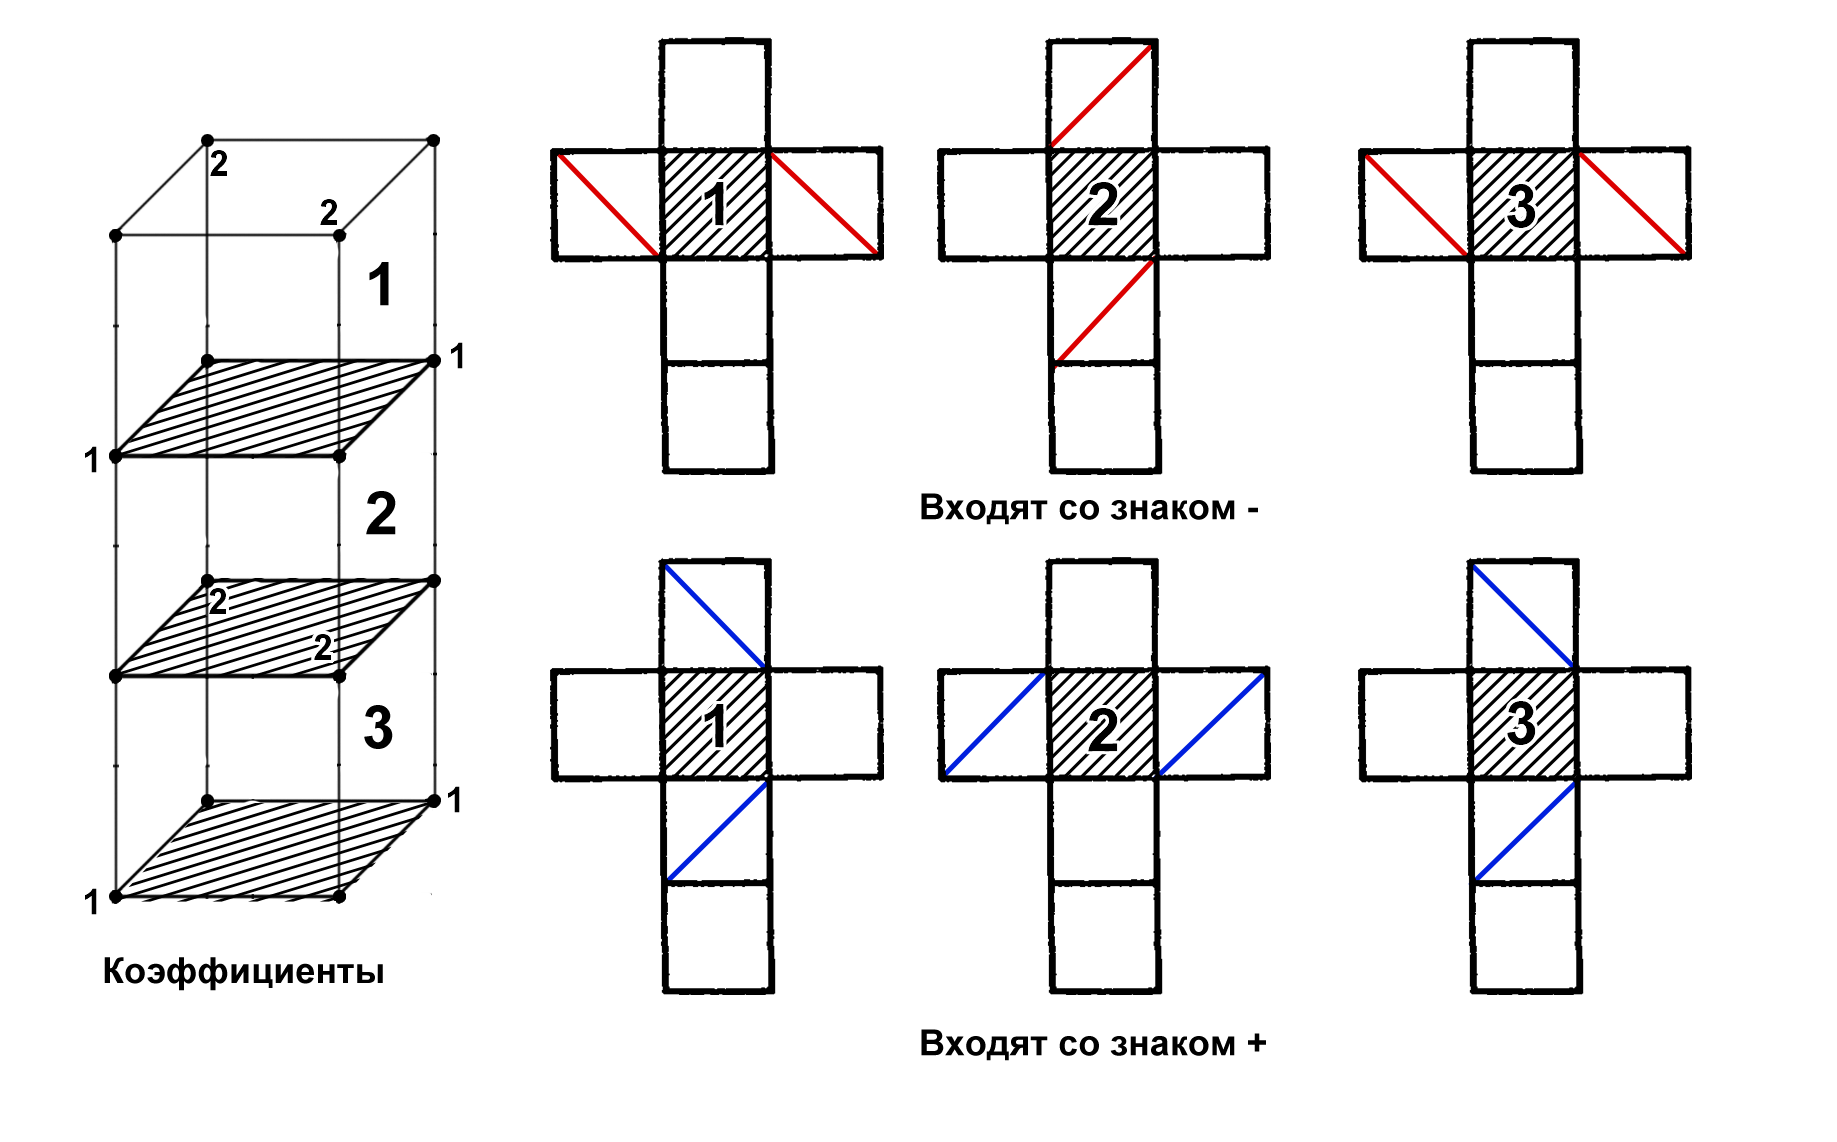
\includegraphics[scale=0.20]{PTS.png}
\caption{}
\label{}
\end{figure}

\begin{figure}[htp]
\centering
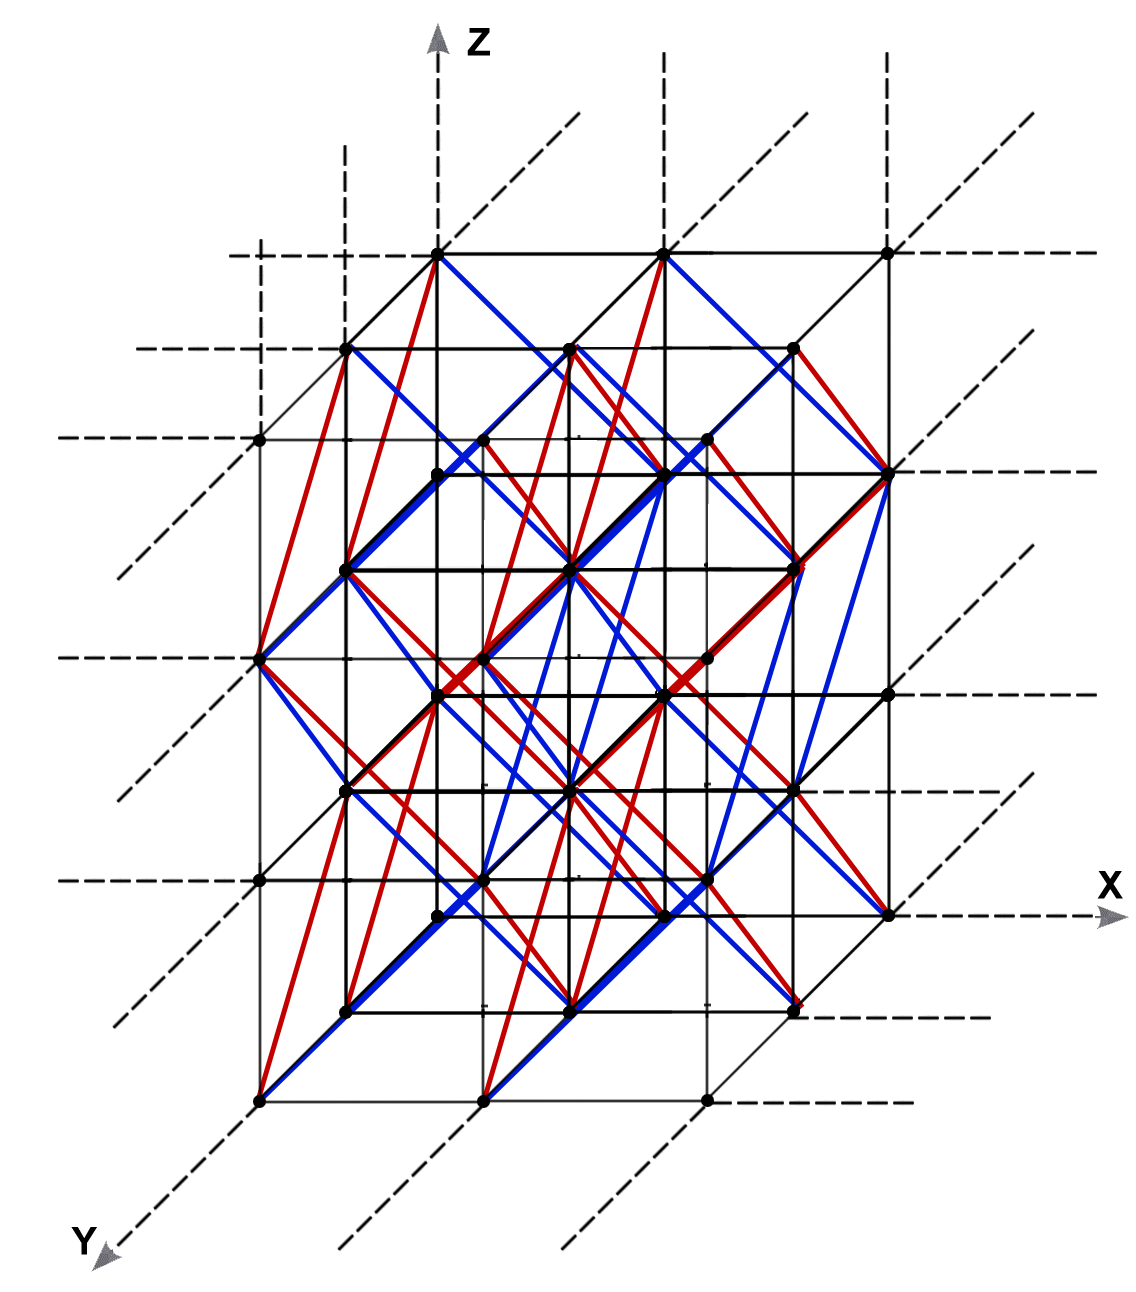
\includegraphics[scale=9.0]{ZELEM.png}
\caption{}
\label{}
\end{figure}

\begin{figure}[htp]
	\centering
	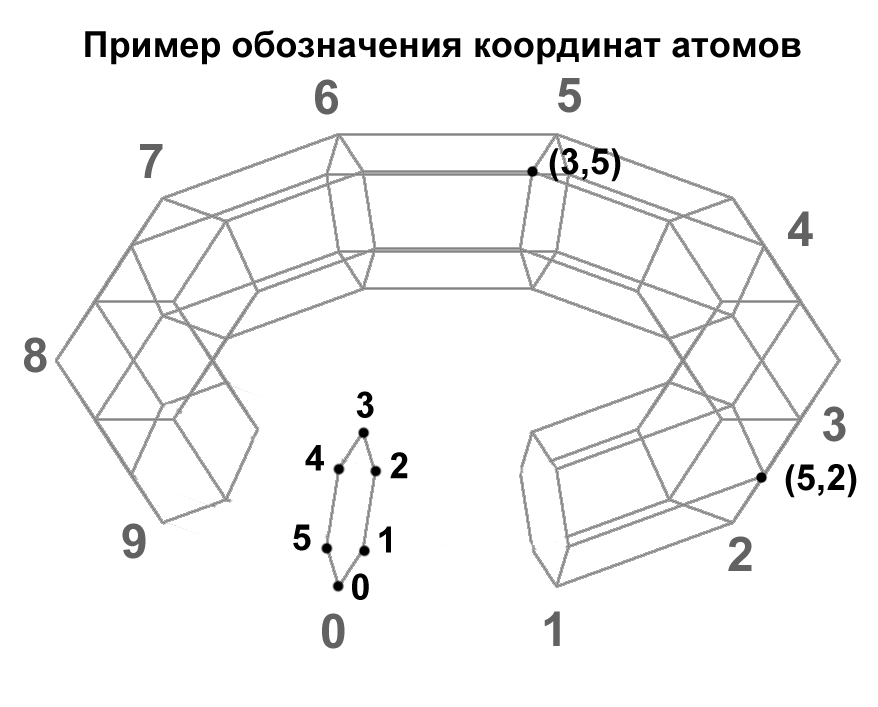
\includegraphics[scale=0.35]{Tor_NUM.png}
	\caption{}
	\label{}
\end{figure}

\newpage
\section{Полученые результаты}
\subsection{Без прилёта фононов}
Графики 4,5:\newline
$N=4$\newline
$M=2$\newline
Вероятности:\newline
$\rho_{000cov+}/\rho_{mol}$ - состояние образованой молекулы\newline
$\rho_{001cov-},\rho_{101cov-}$ - произвольные достижимые состояния\newline
$\sum_{\rho n/d}$ - недостижимые состояния\newline
$\rho_{cov-}$ - состояния без ковалентной связи\newline
\begin{figure}[htp]
\centering
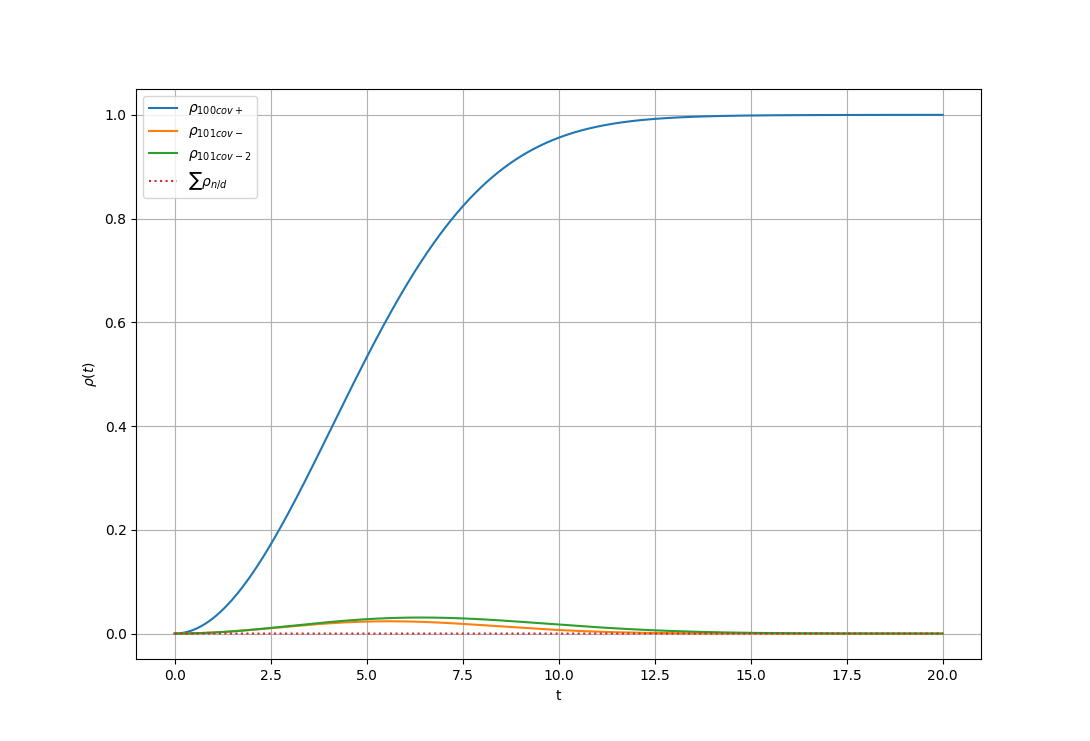
\includegraphics[scale=0.50]{Figure_1.png}
\caption{}
\label{}
\end{figure}
\begin{figure}[htp]
\centering
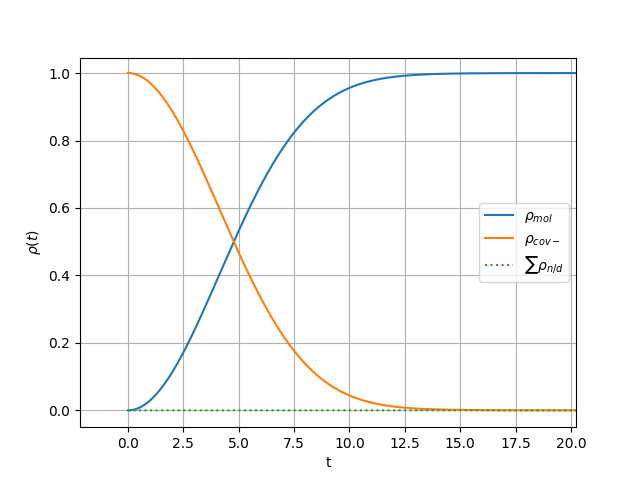
\includegraphics[scale=0.70]{Figure_3.png}
\caption{}
\label{}
\end{figure}
\newpage
\subsection{С прилётом фононов}
Графики 6(7):\newline
$N=4(5)$\newline
$M=2(2)$\newline
Вероятности:\newline
$cov+$ - состояния с ковалентной связью\newline
$cov-$ - состояния без ковалентной связи\newline
\null
\begin{figure}[htp]
\centering
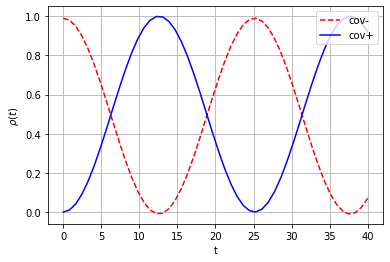
\includegraphics[scale=0.70]{PLT3.png}
\caption{}
\label{}
\end{figure}
\begin{figure}[htp]
\centering
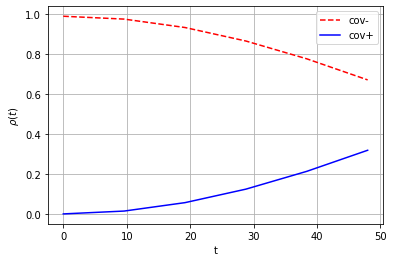
\includegraphics[scale=0.70]{PLT4.png}
\caption{}
\label{}
\end{figure}
\null
\newpage
\subsection{Тороидные решетки}
График 9:\newline
Тороид 4x5\newline
Вероятности:\newline
$\rho_{mol}$ - начальное сотояние [219]*1 (лексиикографический порядок)
\newline
$\rho_{molD}$ - начальное состояние из (Рис. 10)\newline
\begin{figure}[htp]
\centering
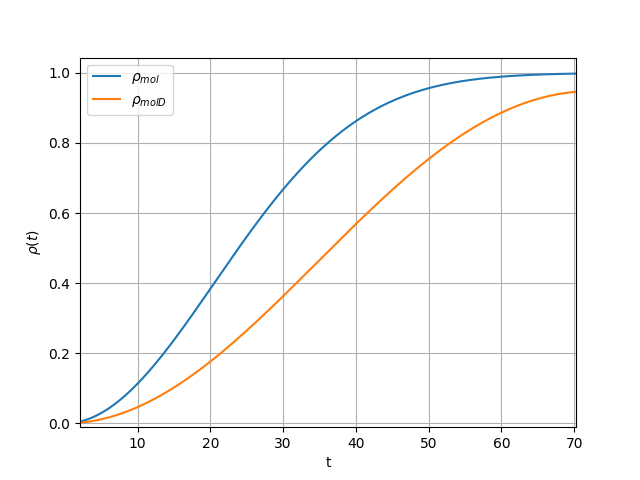
\includegraphics[scale=0.65]{Figure_6.png}
\caption{}
\label{}
\end{figure}
\begin{figure}[htp]
	\centering
	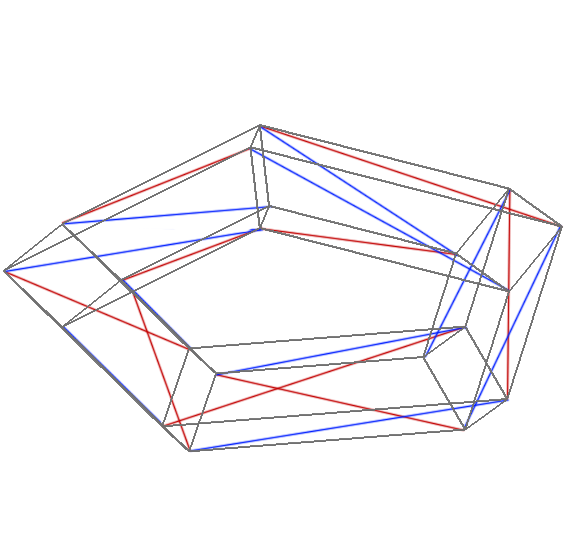
\includegraphics[scale=0.35]{Tor_4_5.png}
	\caption{}
	\label{}
\end{figure}
\newpage

\section{Вычислительная сложность алгоритма}
\subsection{Тороид}
-
\section{Выводы}
-
\section{Список использованной литературы}
\begin{enumerate}
\item Квантовый компьютер / Ю.И. Ожигов. 2020. - 172 с.
\item Фейнмановские лекции по физике / Р. Фейнман, Р. Лейтон, М. Сэндс. 1963.
\item Quantum computations (course of lectures) / Yuri I. Ozhigov
\item Gorini V., Kossakowski A., Sudarshan E. C. G. Completely positive dynamical semigroups of N-level systems // J. Math. Phys. — 1976
\item  Lindblad G. On the generators of quantum dynamical semigroups, // Commun. Math. Phys. — 1976
\item Ландау Л. Д., Лифшиц Е. М. Квантовая механика (нерелятивистская теория). — Издание 4-е. — М.: Наука — 1989.
\item Schrödinger, E. "An Undulatory Theory of the Mechanics of Atoms and Molecules" — 1926
\item H. H. Rosenbrock, "Some general implicit processes for the numerical solution of differential equations", The Computer Journal — 1963 
\item H. Padé. Sur la représentation approchée d’une fonction par des fractions rationnelles Thèse de Doctorat présentée à l’Université de la Sorbonne — 1892

\end{enumerate}
\section{Приложения}
\subsection{Приложение 1}
Функция проверки валидности состояний, вызывая её в цикле нумеруем все достижимые состояния и передаём в другую программу для расчёта динамики (Приложение 2).
\begin{lstlisting}
{

    if (i==j) return (states[i].phx+states[i].phy+
    states[i].phz+states[i].cov)*hW;
    if ((states[i].phx+states[i].phy+states[i].phz)
    <(states[j].phx+states[j].phy+states[j].phz))
        return 0;
    if ((states[j].cov==1)&&((abs(states[i].ax)
    +abs(states[i].ay)+abs(states[i].az))==1))
        if (((states[j].phx<states[i].phx)&&states[i].cov
        ==0&&states[j].ax==1)
          ||((states[j].phy<states[i].phy)&&states[i].cov
          ==0&&states[j].ay==1)
          ||((states[j].phz<states[i].phz)&&states[i].cov
          ==0&&states[j].az==1))
            {
                return Gpho;
            }

    if ((abs(states[i].ax-states[j].ax)
        +abs(states[i].ay-states[j].ay)
        +abs(states[i].az-states[j].az)
        +abs(states[i].phx-states[j].phx)
        +abs(states[i].phy-states[j].phy)
        +abs(states[i].phz-states[j].phz)
        +abs(states[i].cov-states[j].cov))!=1)
        return 0;
    if (((abs(states[i].ax-states[j].ax)+
    abs(states[i].ay-states[j].ay)+
    abs(states[i].az-states[j].az))==1)&&
    ((states[i].cov==states[j].cov)&&states[i].cov==0))
        return Gtun;
    if (states[i].cov!=states[j].cov)
        {
            if ((states[j].cov==1)&&((abs(states[i].ax)+
            abs(states[i].ay)+abs(states[i].az))==1))
                {
                    if((abs(states[i].ax==1)&&(states[i].phx==0))) 
                    	return Gcov;
                    if((abs(states[i].ay==1)&&(states[i].phy==0))) 
                    	return Gcov;
                    if((abs(states[i].az==1)&&(states[i].phz==0))) 
                    	return Gcov;
                }
            if (states[j].cov==0){
                    return 0;
                }
        }
    return 0;
\end{lstlisting}
\subsection{Приложение 2}
Представлен фрагмент программы без улёта фононов
\begin{lstlisting}
rho_ev = []
rho = np.copy(rho_0)
rho_ev.append(rho)

for i in range(1000):
    rho = np.dot(exp_H_m, np.dot(rho, exp_H_p))
    rho = rho + L(rho) * d_tau
    rho_ev.append(rho)

rho_0_ev = []
rho_12_ev = []
....
rho_204_ev = []
rho_212_ev = []

x_mesh = np.linspace(0, (len(rho_ev)-1) * d_tau, len(rho_ev))
for i in range(len(rho_ev)):
    rho_0_ev.append(np.abs(rho_ev[i][0,0]))
    rho_12_ev.append(np.abs(rho_ev[i][12,12]))
    ...
    rho_204_ev.append(np.abs(rho_ev[i][204,204]))
    rho_212_ev.append(np.abs(rho_ev[i][212,212]))
\end{lstlisting}
Выбраны 0,12..204,214 - состояния в которых ковалентная связь образована, далее вычисляется вероятность нахождения в этих состояниях
\end{document}
